% ============================================================
% A.1 Hyperparameter Configuration
% ============================================================
\subsection{Hyperparameter Configuration}
\label{sec:hyperparams}

Table~\ref{tab:hyperparams} lists all hyperparameters used in the heuristic functions and search algorithms. Values are fixed across all experiments unless otherwise noted.

\begin{table}[h]
\centering
\small
\caption{Hyperparameters and their values.}
\label{tab:hyperparams}
\begin{tabular}{llc}
\toprule
\textbf{Parameter} & \textbf{Description} & \textbf{Value} \\
\midrule
\multicolumn{3}{l}{\textit{H1 -- Liquidity Heuristic}} \\
$\lambda_{\text{liq}}$ & Liquidity penalty weight & 1.0 \\
Unknown penalty & No-data fallback cost & 5.0 \\
Cache TTL & Volume cache lifetime & 60\,s \\
\midrule
\multicolumn{3}{l}{\textit{H2 -- Slippage Heuristic}} \\
$\lambda_{\text{slip}}$ & Slippage penalty weight & 0.5 \\
$\theta$ & Slippage tolerance & 10\,bps \\
Unknown penalty & No-data fallback cost & 50.0 \\
Cache TTL & Order-book cache lifetime & 30\,s \\
\midrule
\multicolumn{3}{l}{\textit{H4 -- Chain/Exchange Risk}} \\
$\lambda_{\text{chain}}$ & Chain risk penalty weight & 1.0 \\
$\lambda_{\text{exchange}}$ & Exchange risk penalty weight & 1.0 \\
$w_{\min}$ & Min Weighted A* weight & 1.0 \\
$w_{\max}$ & Max Weighted A* weight & 3.0 \\
\midrule
\multicolumn{3}{l}{\textit{Search Parameters}} \\
Max depth & Maximum path hops & 6 \\
$T_{\max}$ & Arbitrage time window & 1800\,s \\
Early exit iter. & Iters after first profit & 200 \\
$k$ (H3) & Multi-start parallel runs & 3 \\
User overhead & Execution latency per hop & 45\,s \\
\bottomrule
\end{tabular}
\end{table}

\paragraph{Chain transfer times.}
Transfer-time estimates are drawn from documented blockchain finality times plus typical exchange processing delays: Solana $\approx$~1\,s, BNB Chain $\approx$~4\,s, Polygon $\approx$~5\,s, Tron $\approx$~30\,s, Arbitrum/Base $\approx$~120\,s, Ethereum L1 $\approx$~600\,s. These are used by $h_4$ to compute chain reliability penalties and by the transfer-time model to assess path time-feasibility.

\paragraph{Exchange reliability scores.}
Each exchange is assigned a static reliability score $s(n) \in [0,1]$ based on historical uptime, withdrawal availability, and community reports. Higher scores indicate more reliable exchanges. These scores are pre-computed and cached, requiring zero API calls during search.

% ============================================================
% A.2 Ethics and Broader Impact
% ============================================================
\subsection{Ethics and Broader Impact}
\label{sec:ethics_appendix}

\paragraph{Data and privacy.}
This work uses only publicly available market data (prices, order books, fee schedules) accessed through CCXT. No proprietary, personal, or user-specific data are collected or used.

\paragraph{Market impact.}
Arbitrage activity generally improves market efficiency by reducing cross-exchange price discrepancies. However, large-scale automated arbitrage could theoretically contribute to flash crashes or liquidity draining in thin markets. Our framework operates at order sizes (\$100--\$100k) that are small relative to exchange daily volumes (\$100M+) and is designed as a research prototype, not a production trading system.

\paragraph{Environmental considerations.}
Our framework queries exchange APIs and performs lightweight graph search computations. It does not execute on-chain transactions, mine blocks, or contribute to blockchain energy consumption. The computational footprint is negligible (P99 search time $<$7\,s, even for API-dependent heuristics).

\paragraph{Regulatory compliance.}
Cross-exchange arbitrage operates within established market structures and does not exploit insider information or engage in market manipulation. Users of this framework should comply with applicable financial regulations in their jurisdiction, including exchange terms of service and cryptocurrency trading laws.

% ============================================================
% A.3 Additional Experimental Results
% ============================================================
\subsection{Additional Experimental Results}
\label{sec:additional_results}

\paragraph{Heuristic comparison: expansions and compute time.}
Figure~\ref{fig:app_expansion_time} compares mean node expansions and compute time across all heuristics on the cached graph. $h_2$ consistently achieves the fewest expansions, while $h_4$ matches Dijkstra-class latency due to pre-computed scores requiring zero API calls.

\begin{figure}[h]
\centering
\begin{subfigure}[t]{0.48\textwidth}
    \centering
    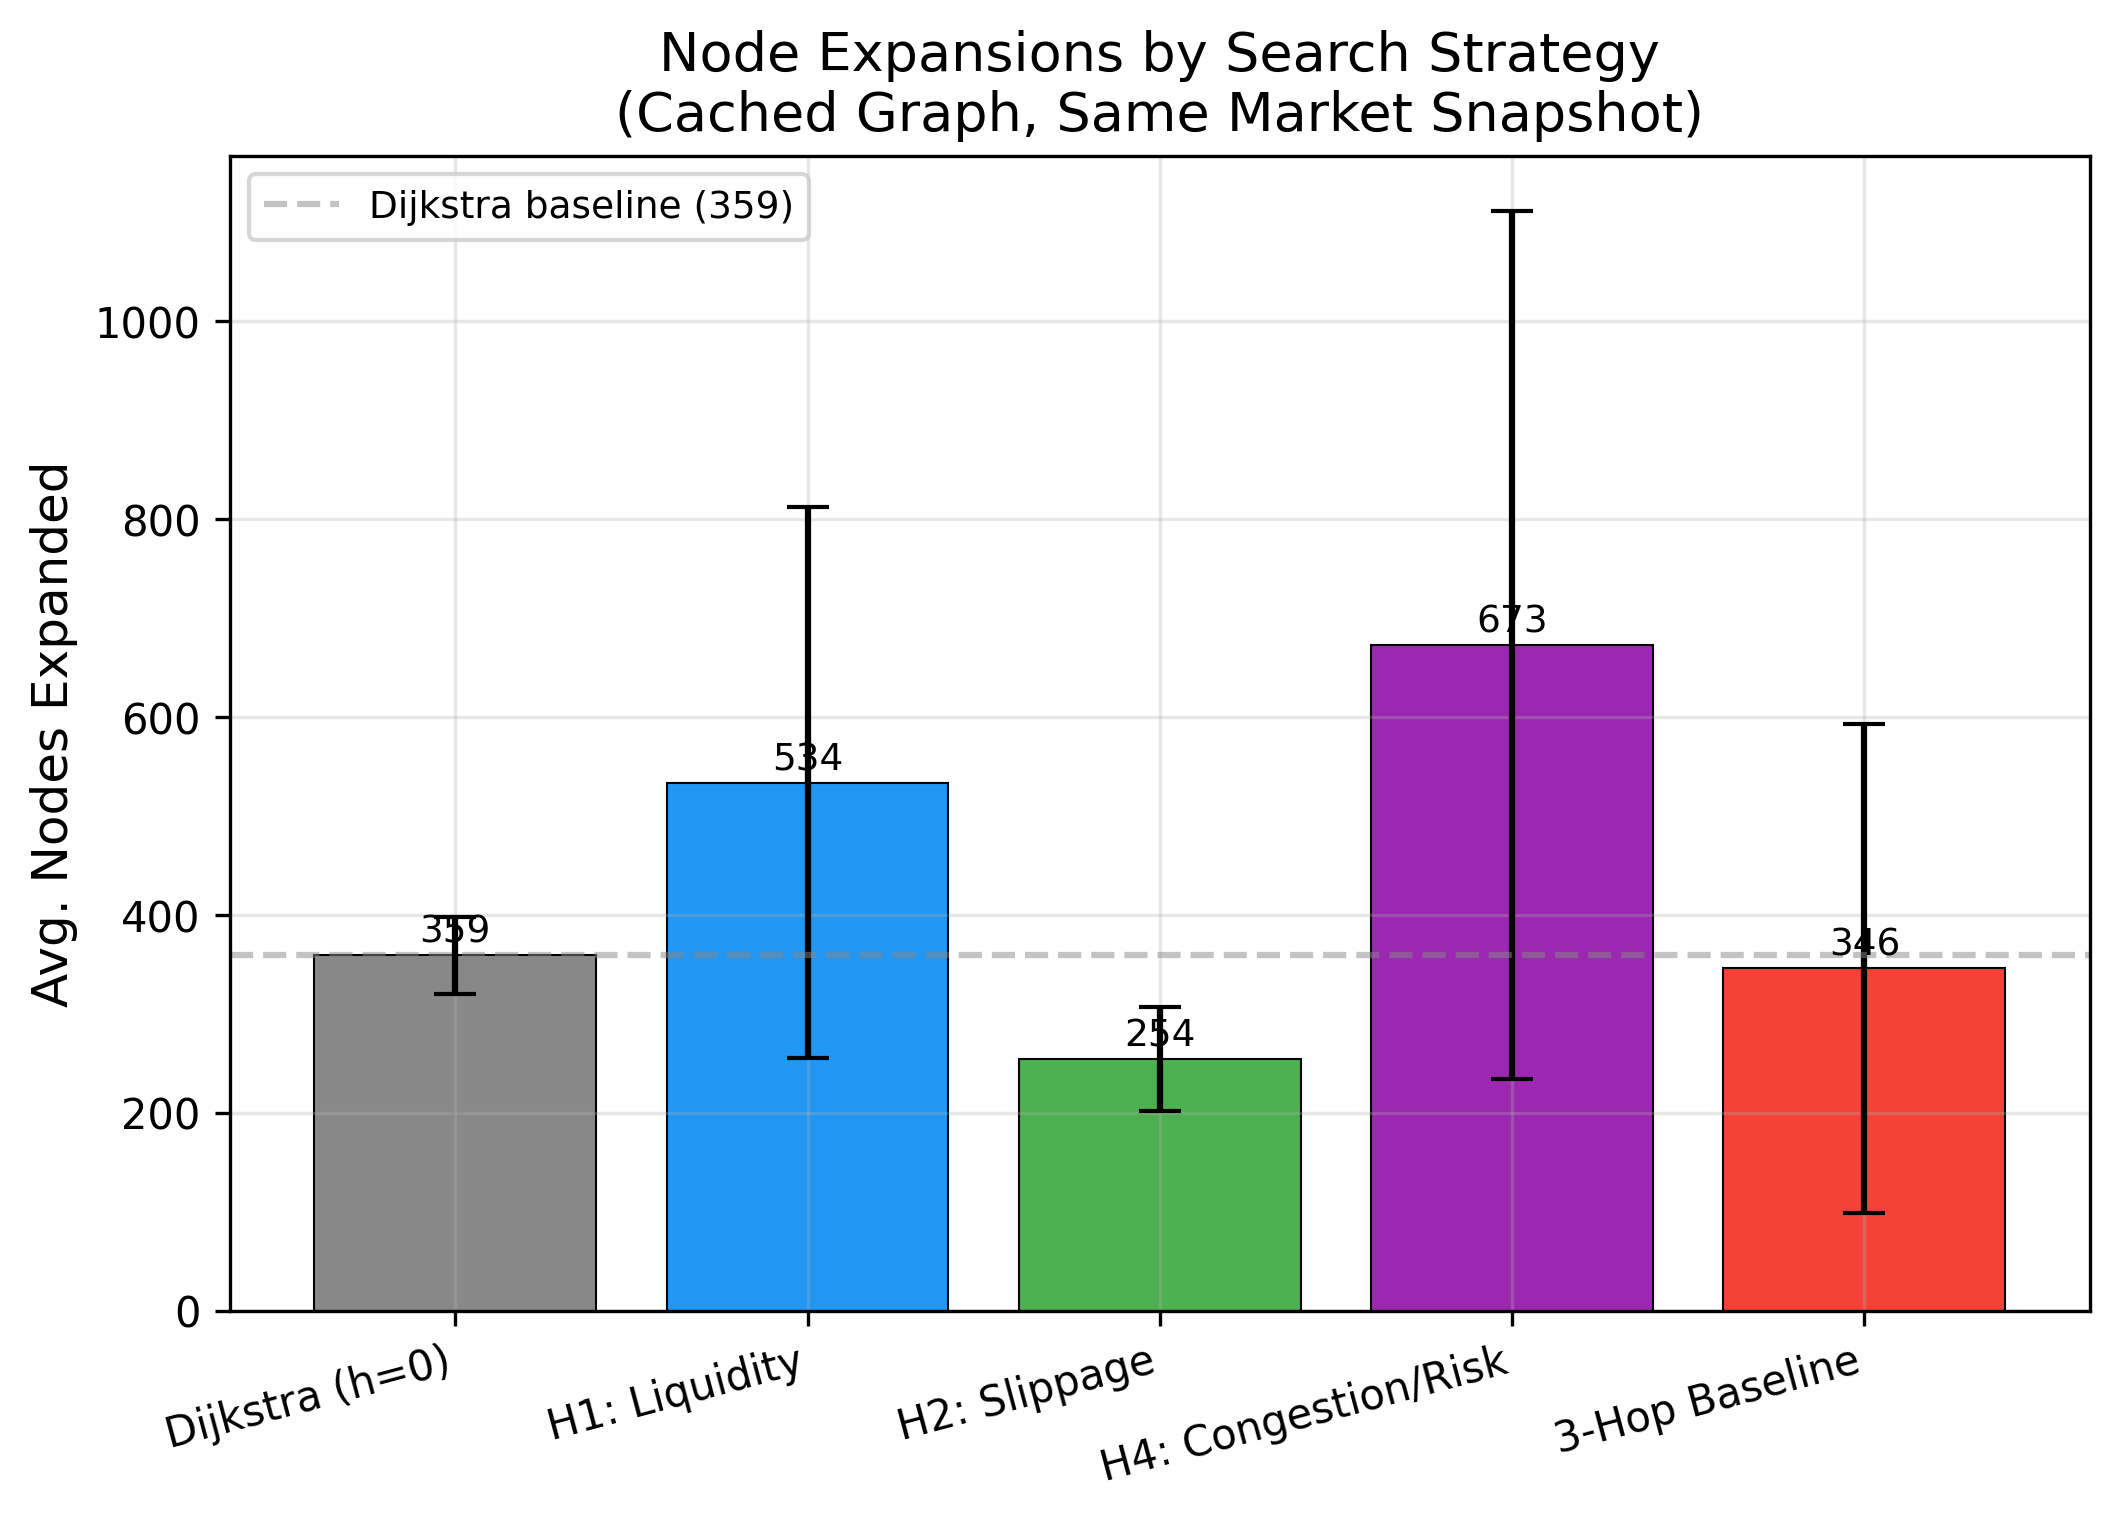
\includegraphics[width=\textwidth]{figures/fig01_node_expansion_bar.png}
    \caption{Mean node expansions by heuristic.}
\end{subfigure}
\hfill
\begin{subfigure}[t]{0.48\textwidth}
    \centering
    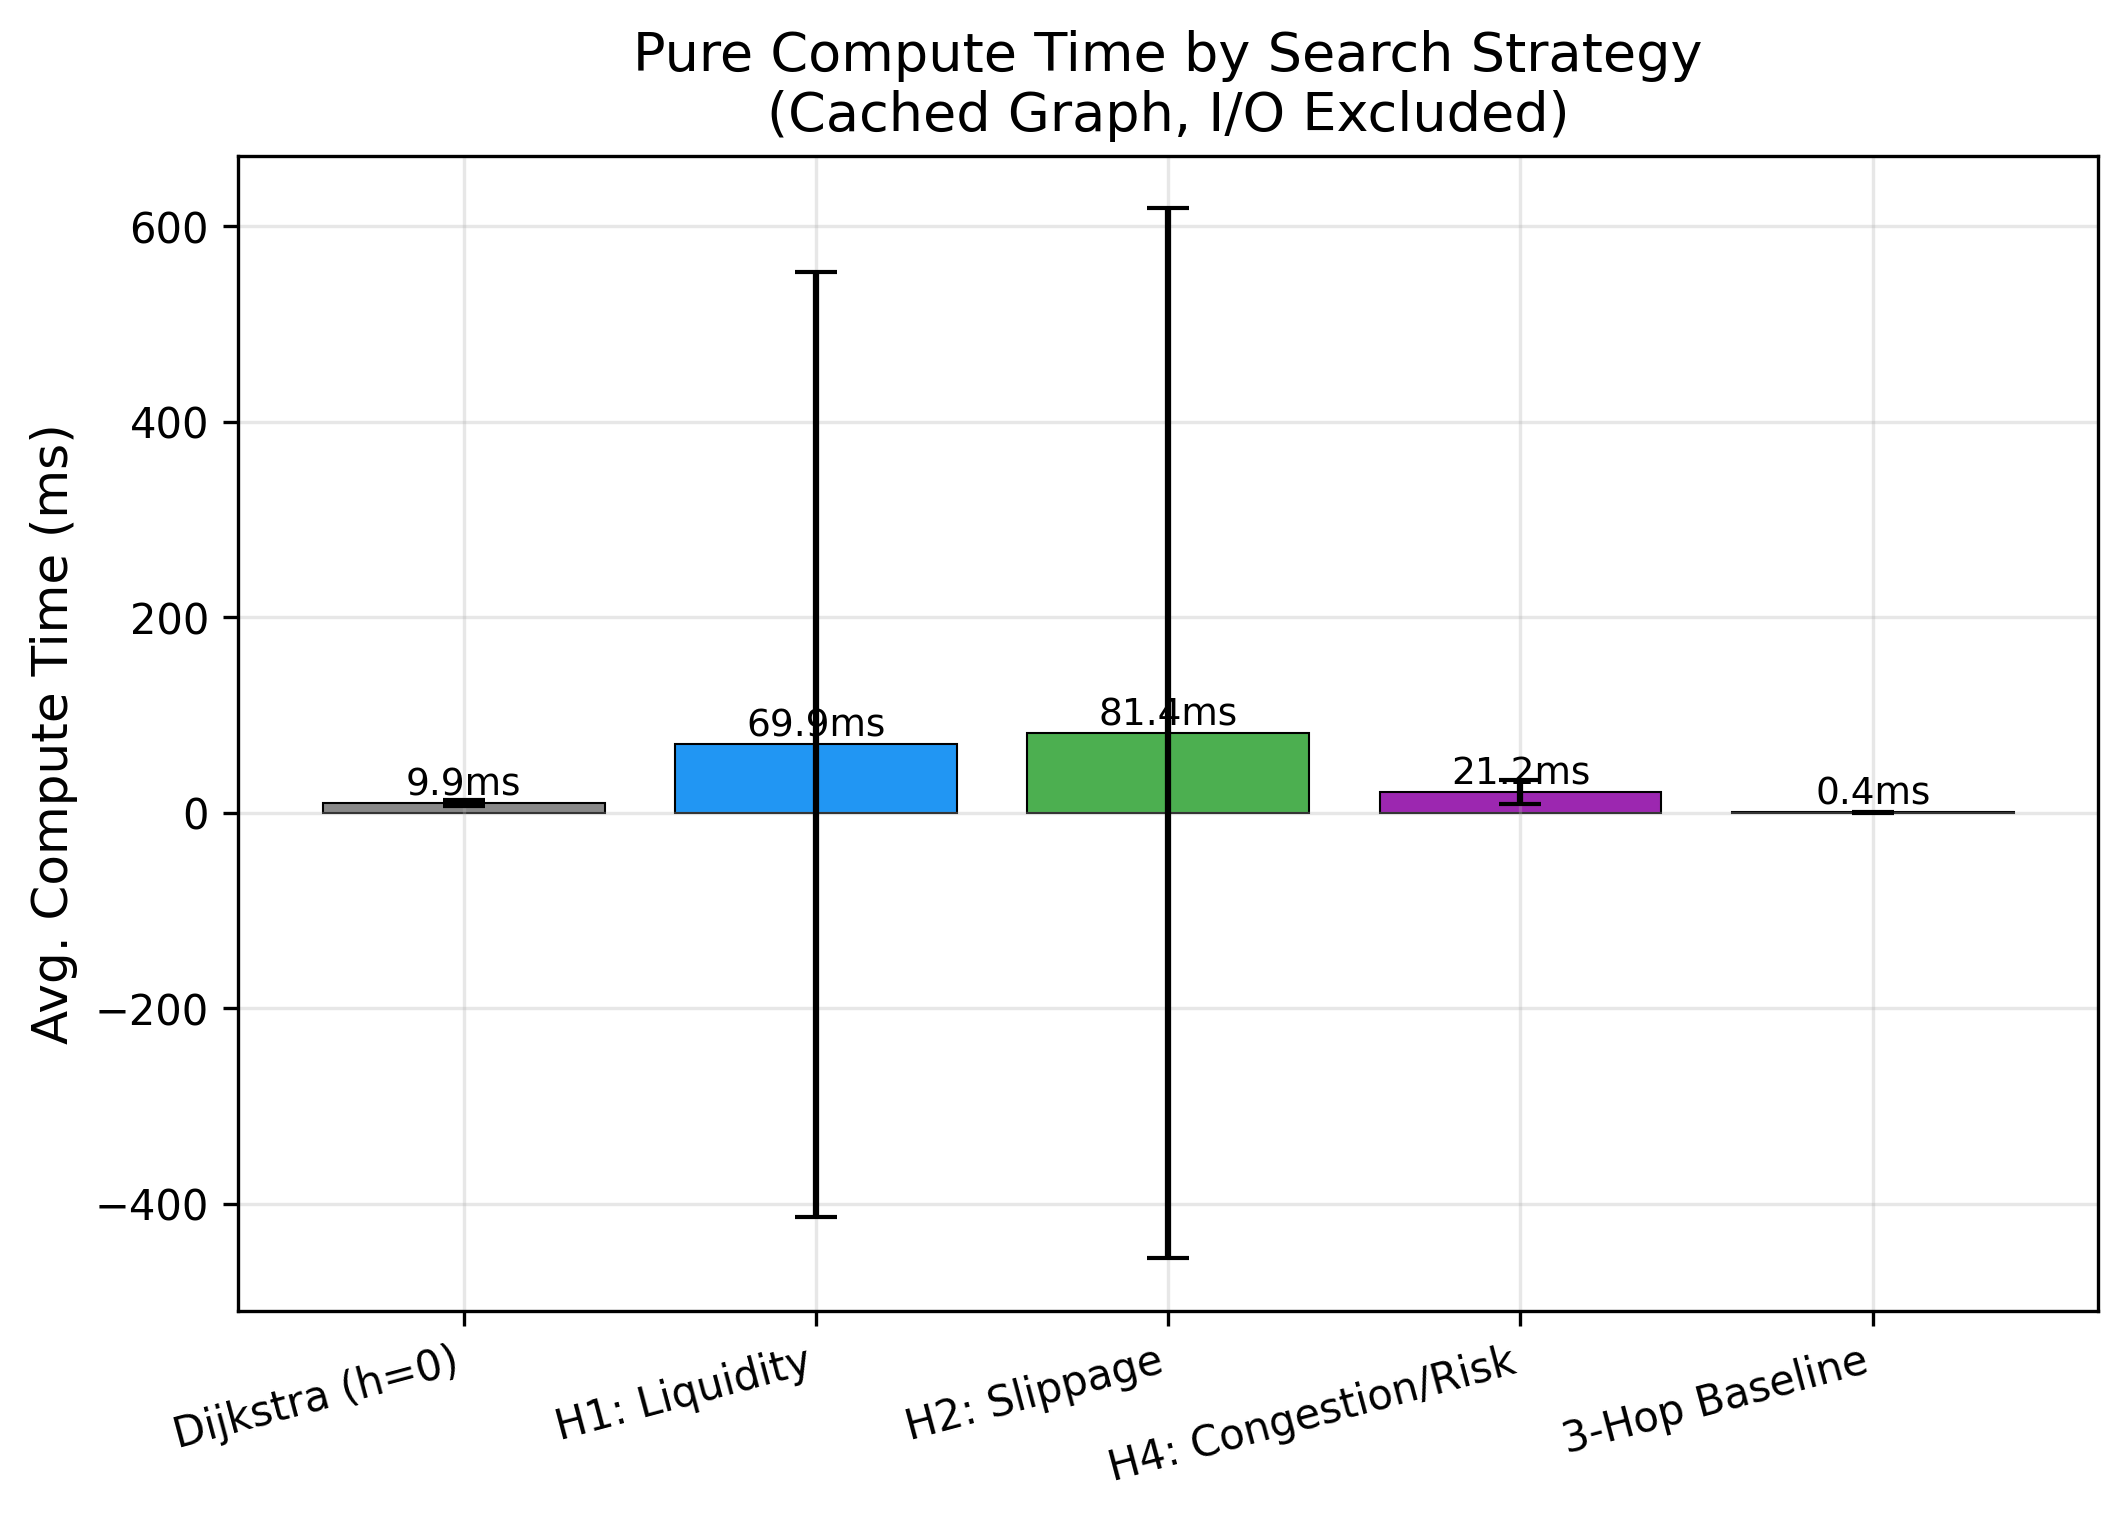
\includegraphics[width=\textwidth]{figures/fig02_compute_time_bar.png}
    \caption{Mean compute time by heuristic.}
\end{subfigure}
\caption{Heuristic comparison on cached graph (30~start nodes, 3~cash levels).}
\label{fig:app_expansion_time}
\end{figure}

\paragraph{Overnight temporal evolution.}
Figure~\ref{fig:app_overnight_ts} shows profit trajectories across 96~snapshots (8~hours, 5-min intervals). Profitable opportunities persist throughout the entire session, with profits clustering around 2--3 structural optima per start node. Periodic dips correspond to temporary market equilibria that resolve within minutes.

\begin{figure}[h]
\centering
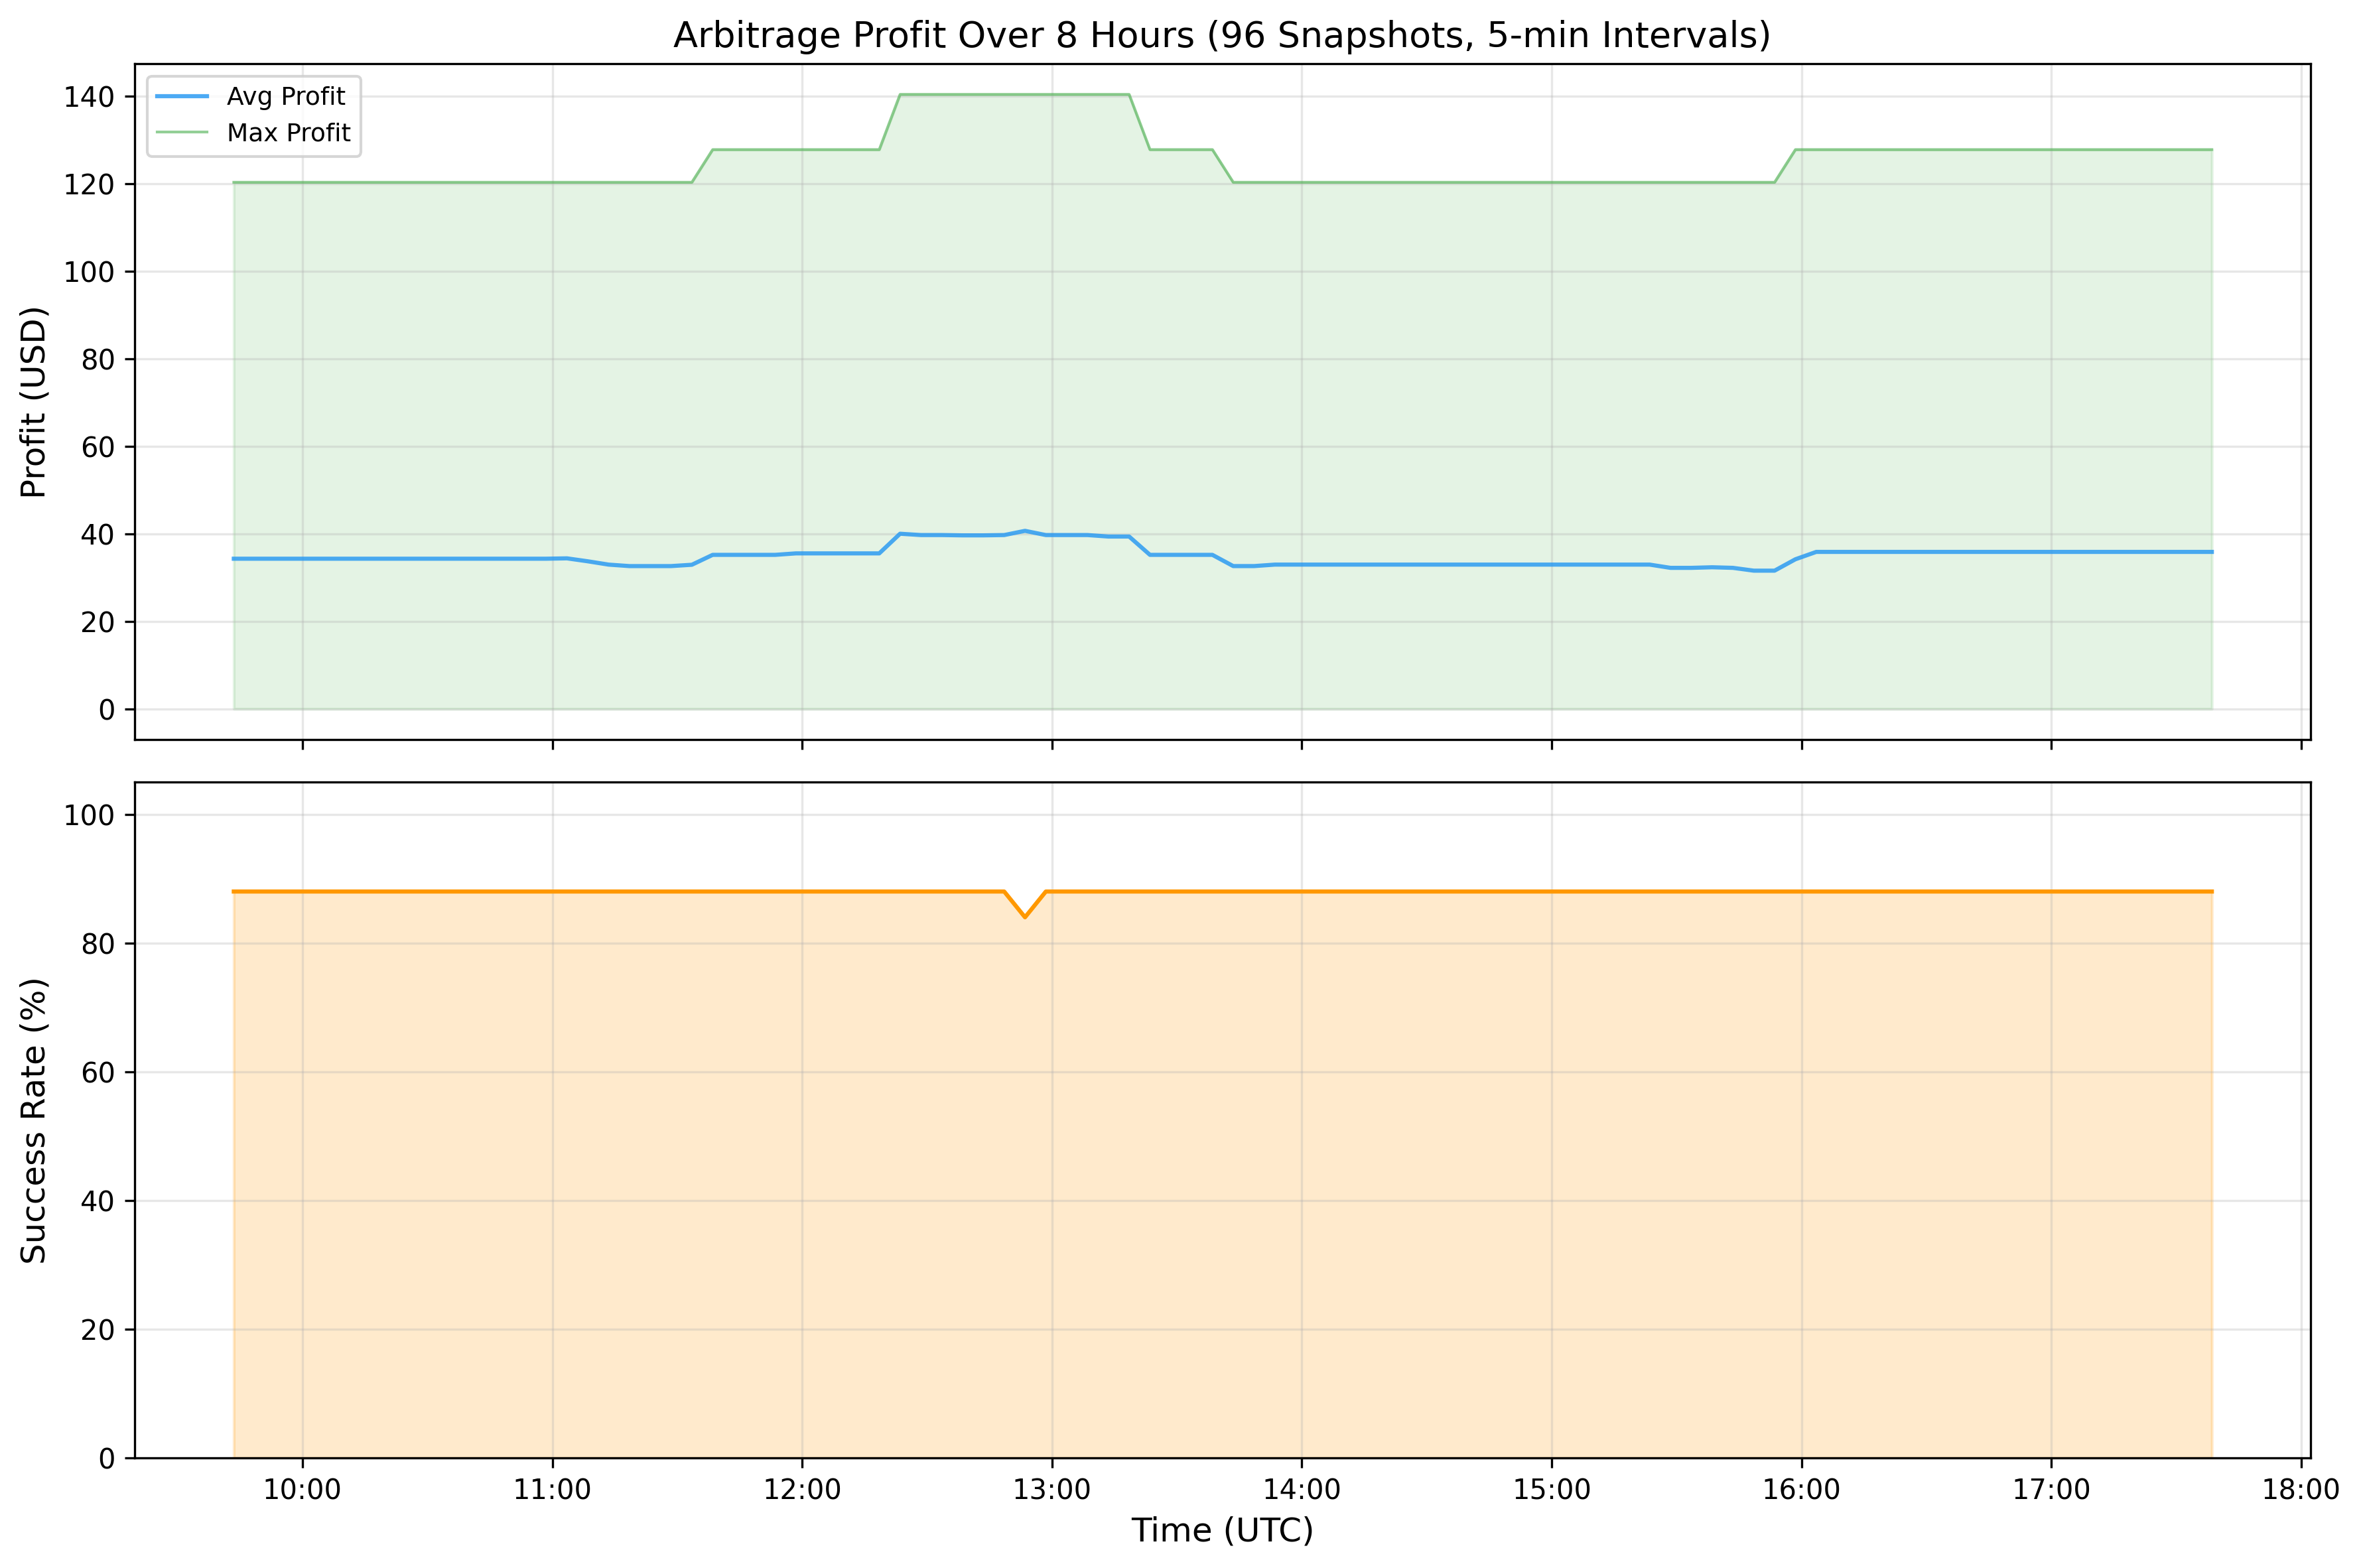
\includegraphics[width=0.85\textwidth]{figures/fig10_overnight_timeseries.png}
\caption{Overnight profit timeseries across all heuristics (8~hours, 5-min intervals, 5~start nodes, 3~cash levels).}
\label{fig:app_overnight_ts}
\end{figure}

\paragraph{Sensitivity: $h_1$ liquidity penalty and max depth.}
Figure~\ref{fig:app_sensitivity_extra} shows that $h_1$ performance is robust across $\lambda_{\text{liq}} \in [0.1, 5.0]$, and that increasing max depth beyond 3 hops yields no additional profit, confirming that profitable stablecoin paths are inherently short.

\begin{figure}[h]
\centering
\begin{subfigure}[t]{0.48\textwidth}
    \centering
    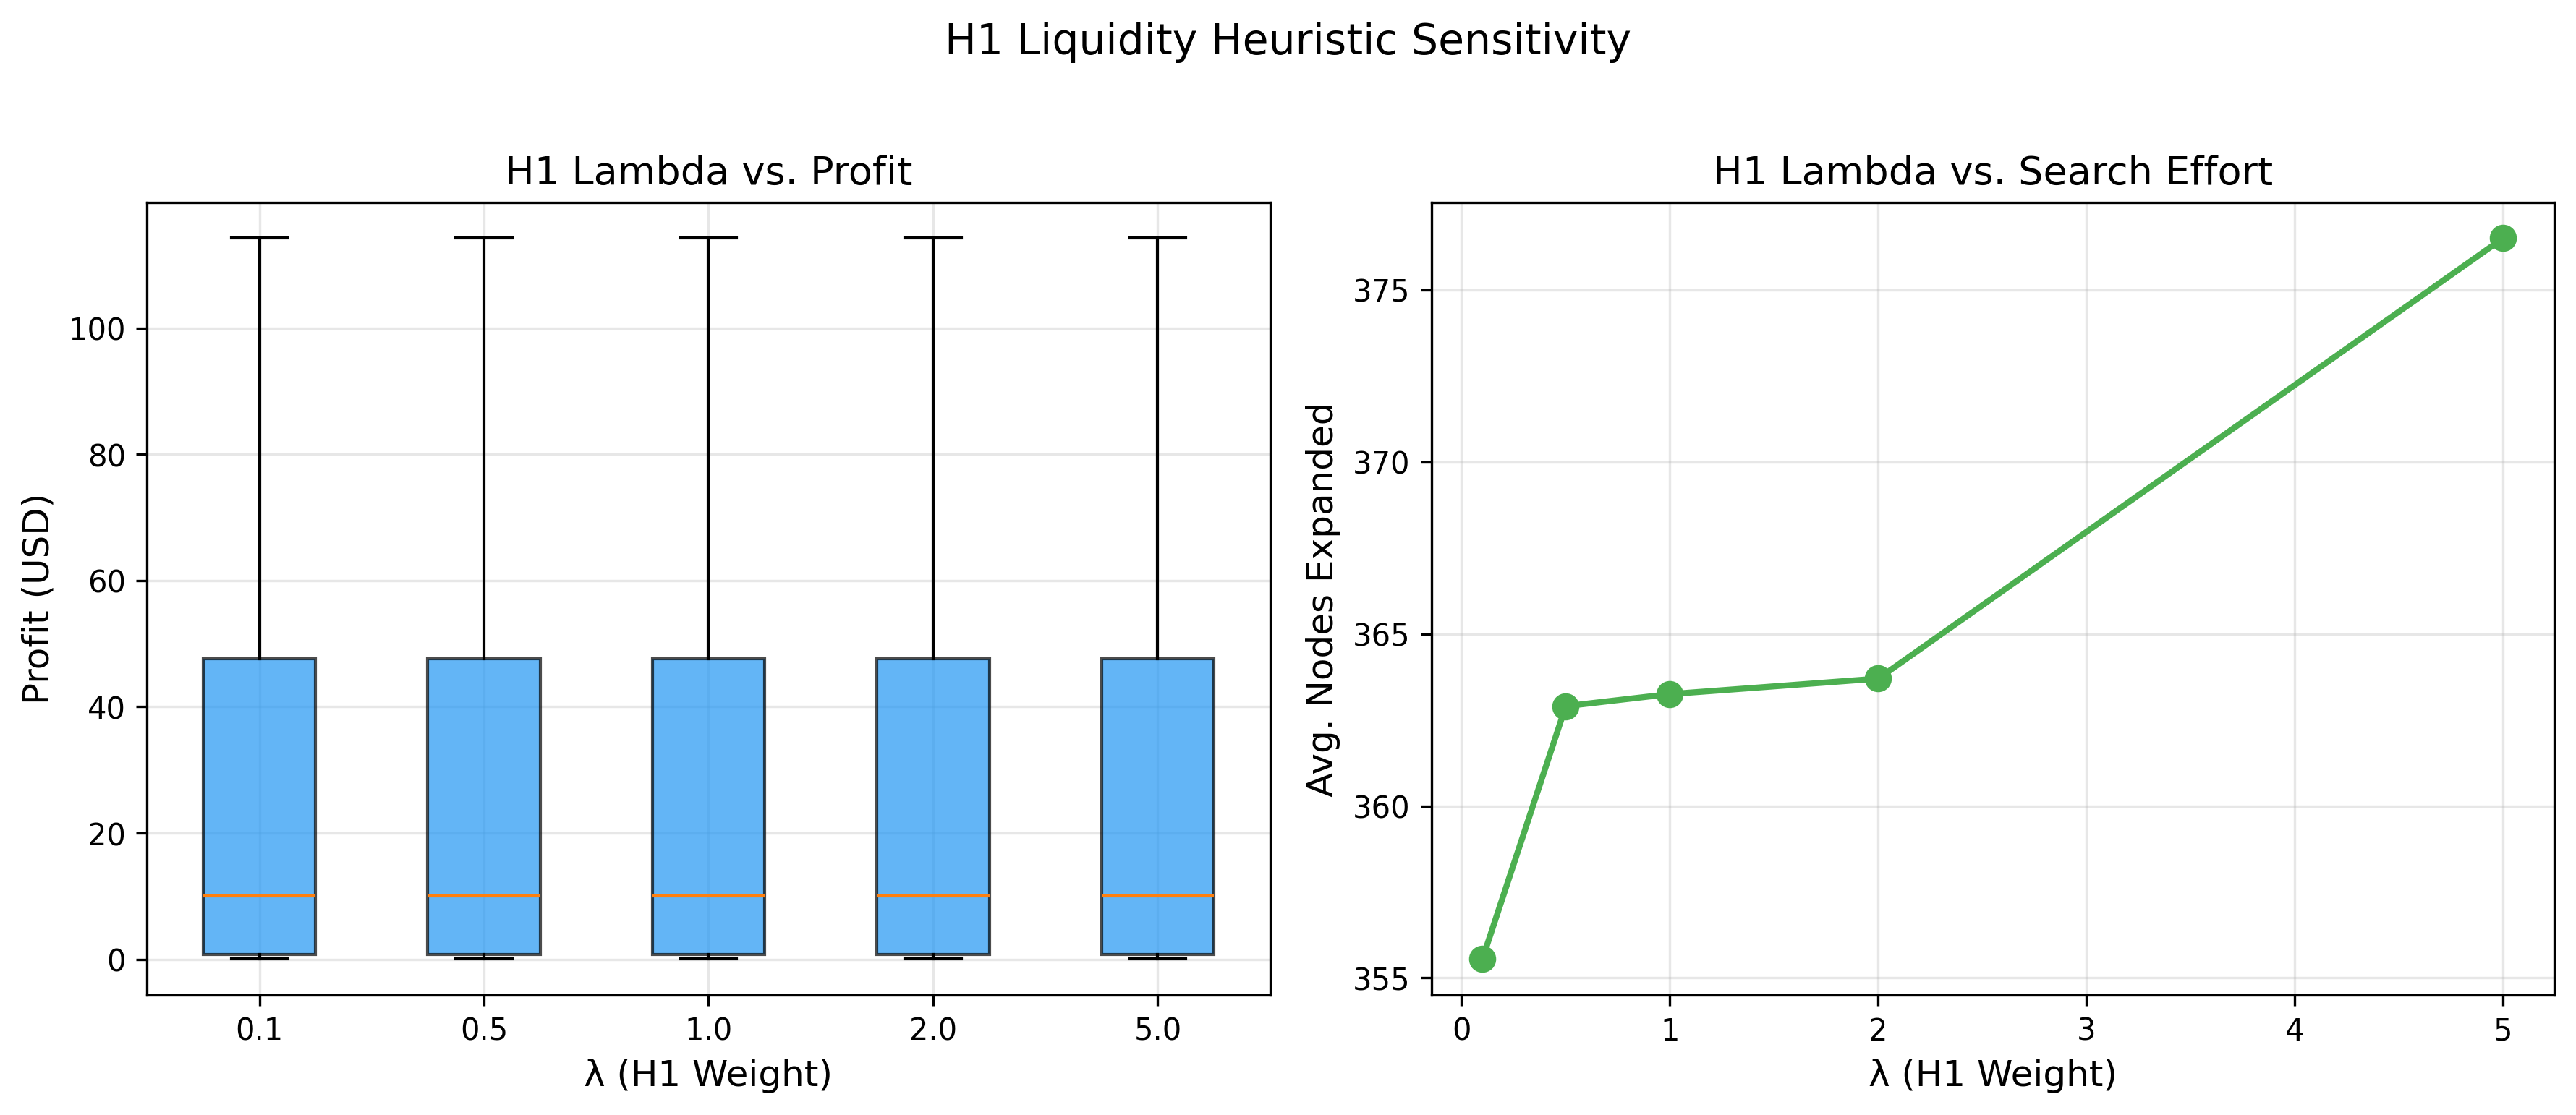
\includegraphics[width=\textwidth]{figures/fig12_sensitivity_h1_lambda.png}
    \caption{$h_1$: profit vs.\ $\lambda_{\text{liq}}$.}
\end{subfigure}
\hfill
\begin{subfigure}[t]{0.48\textwidth}
    \centering
    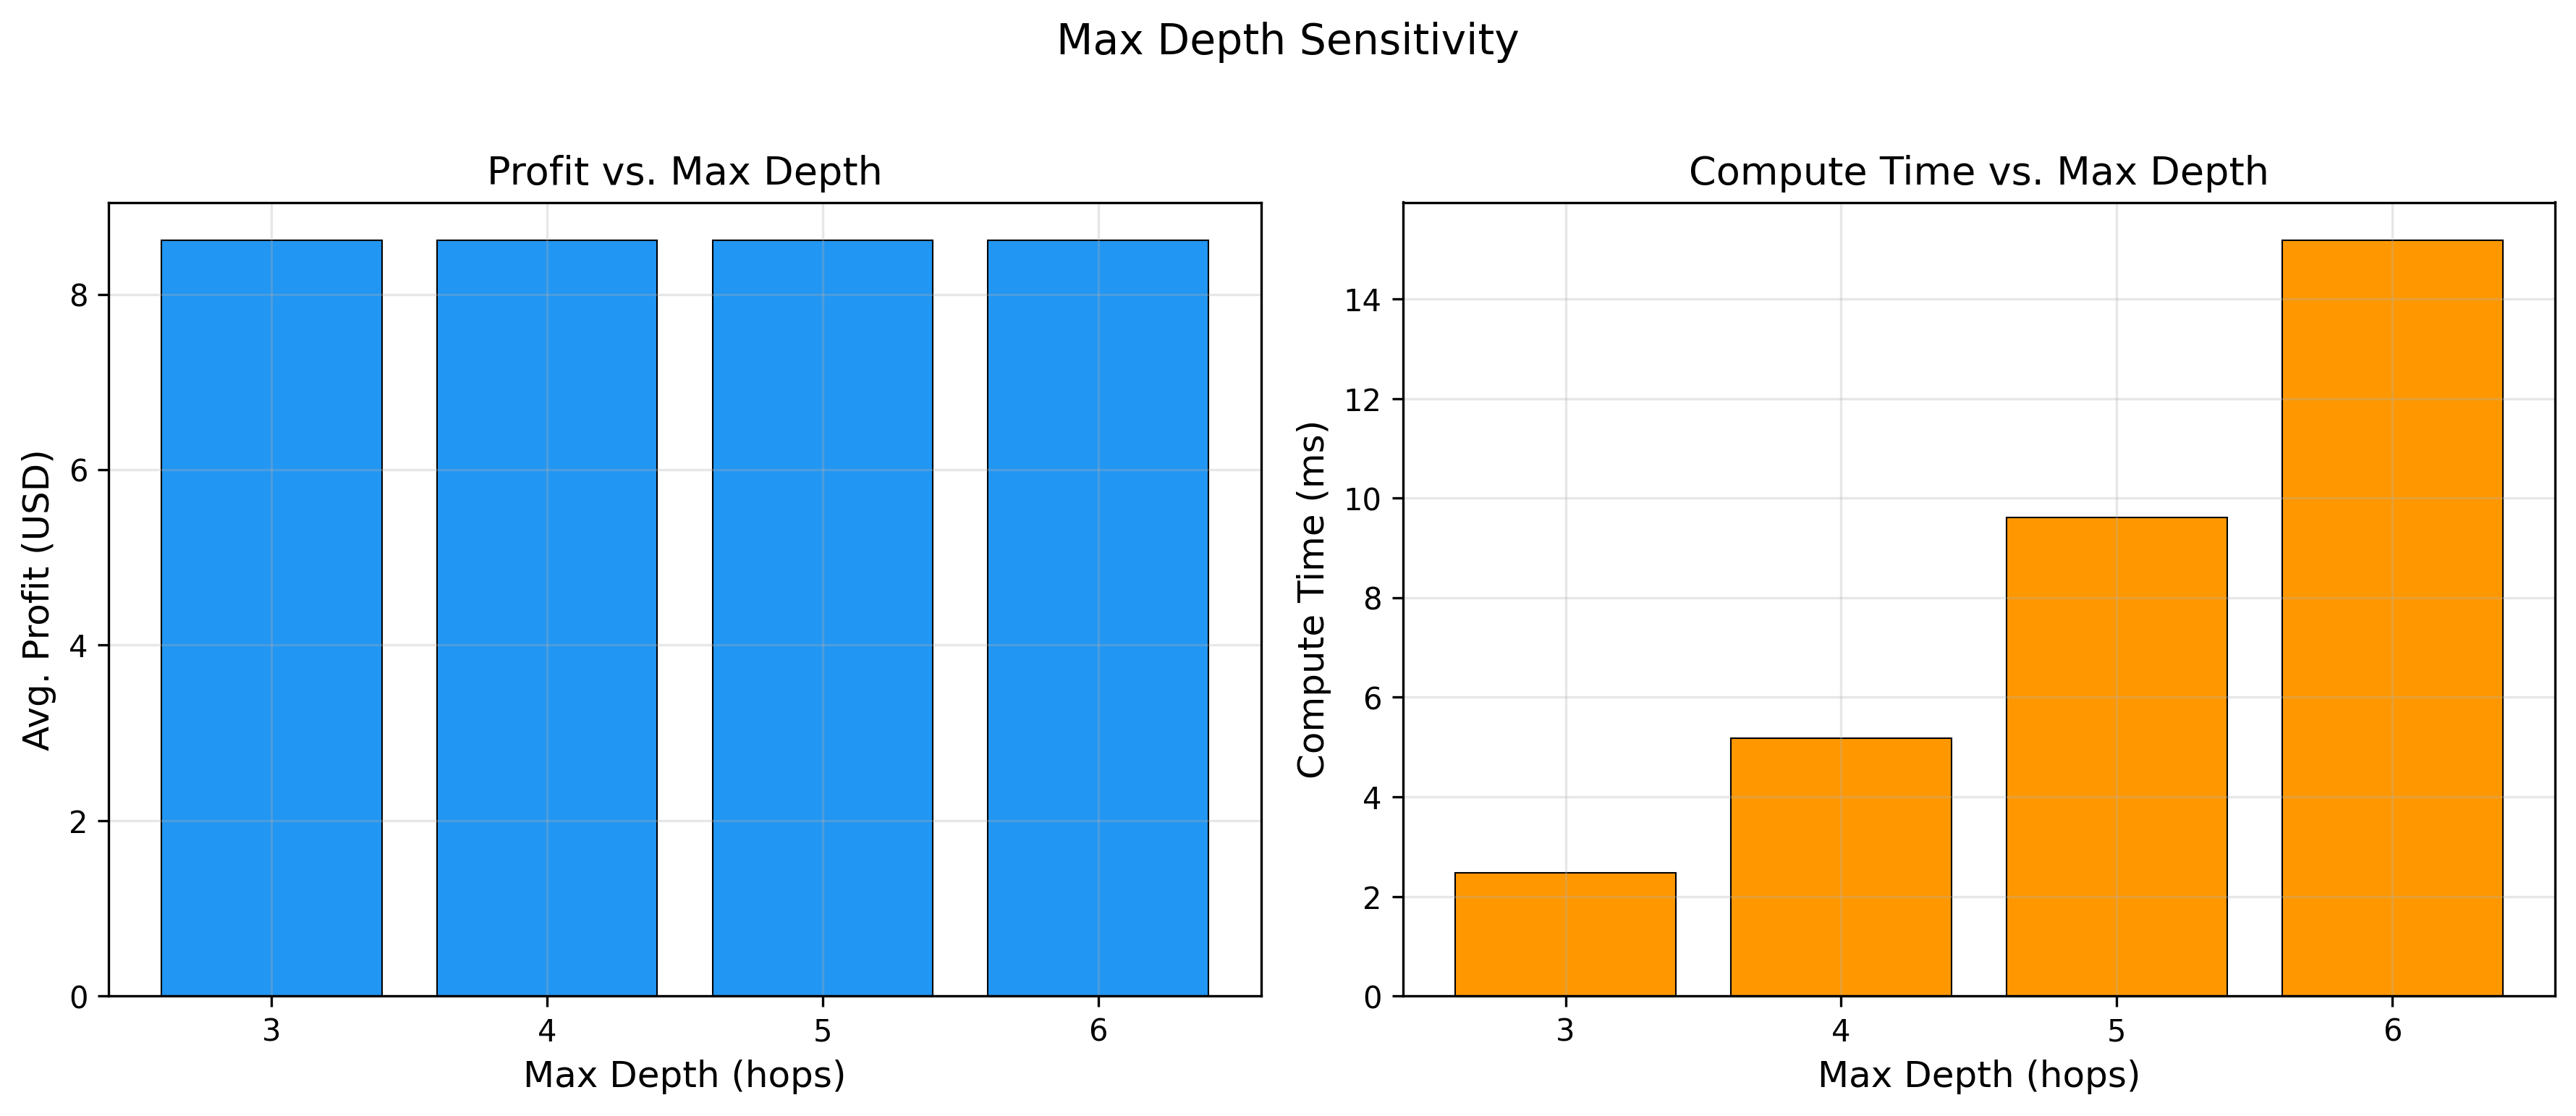
\includegraphics[width=\textwidth]{figures/fig15_sensitivity_max_depth.png}
    \caption{Profit vs.\ max path depth.}
\end{subfigure}
\caption{Additional sensitivity analysis.}
\label{fig:app_sensitivity_extra}
\end{figure}

\paragraph{Radar summary and profit distribution.}
Figure~\ref{fig:app_radar_profit} provides a multi-dimensional summary of heuristic performance across six metrics, alongside the profit distribution across order sizes. $h_4$ dominates on speed and reliability, while $h_2$ leads on expansion efficiency.

\begin{figure}[h]
\centering
\begin{subfigure}[t]{0.48\textwidth}
    \centering
    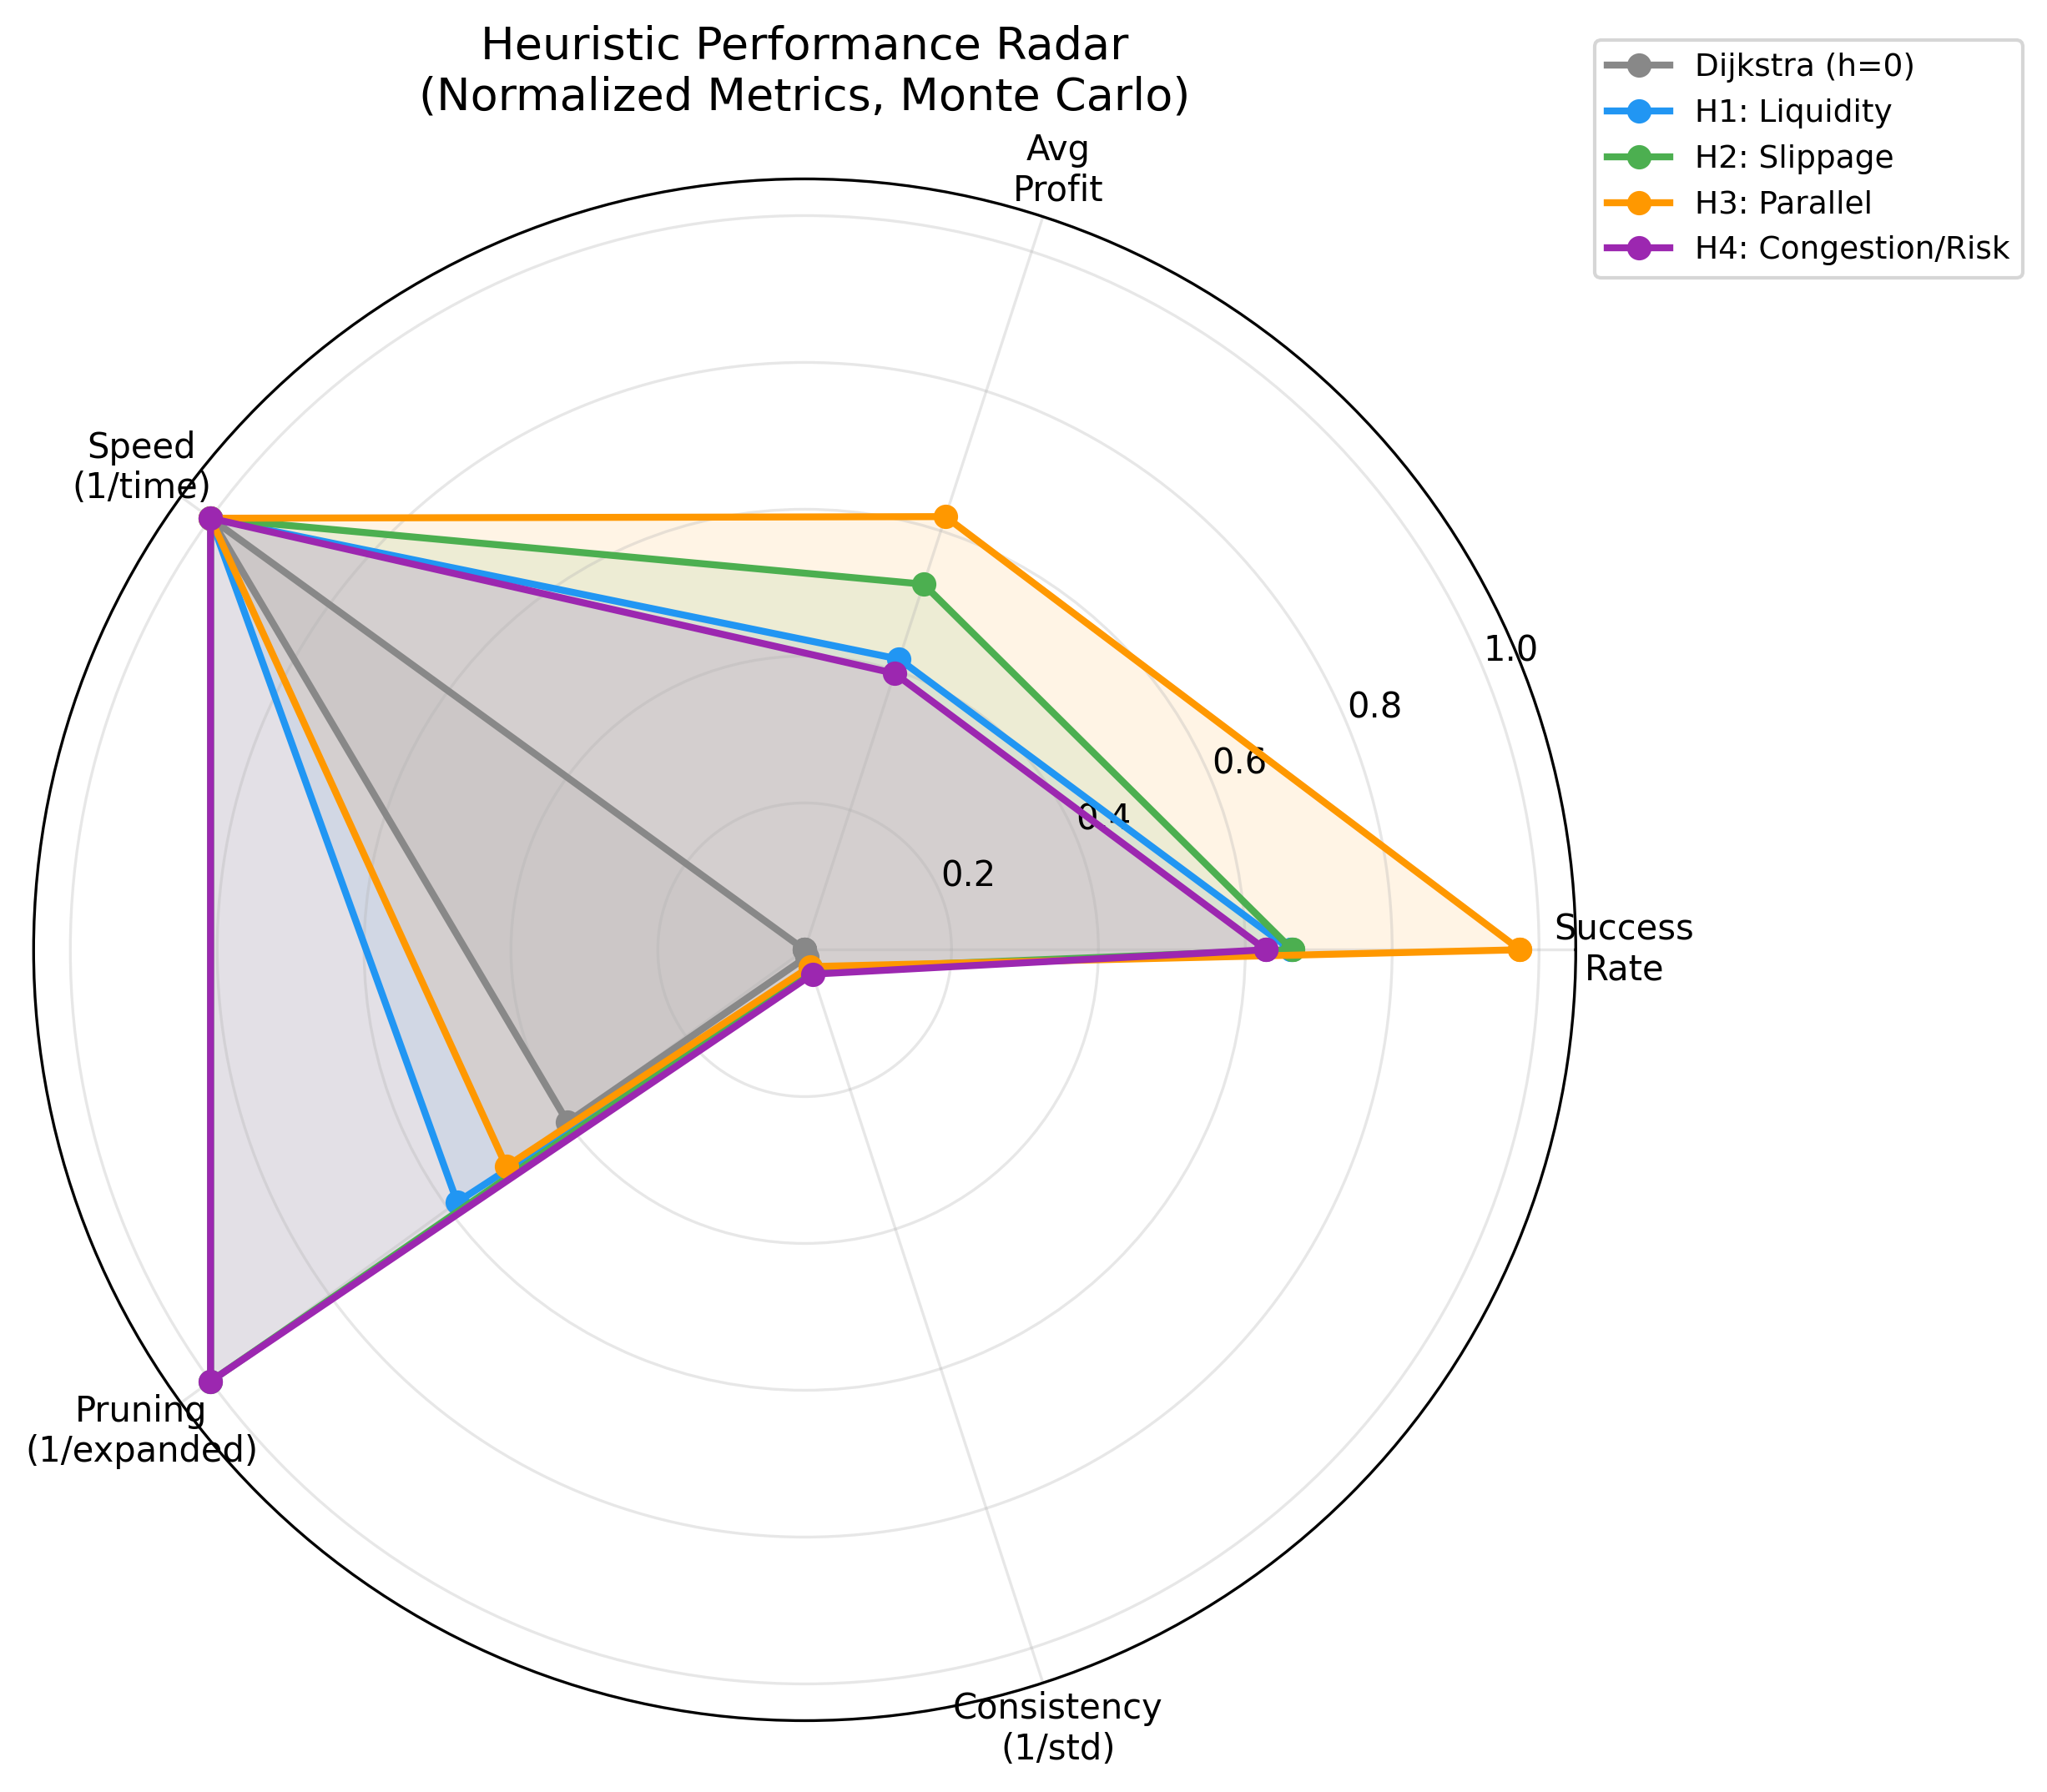
\includegraphics[width=\textwidth]{figures/fig18_radar_summary.png}
    \caption{Radar: multi-metric heuristic comparison.}
\end{subfigure}
\hfill
\begin{subfigure}[t]{0.48\textwidth}
    \centering
    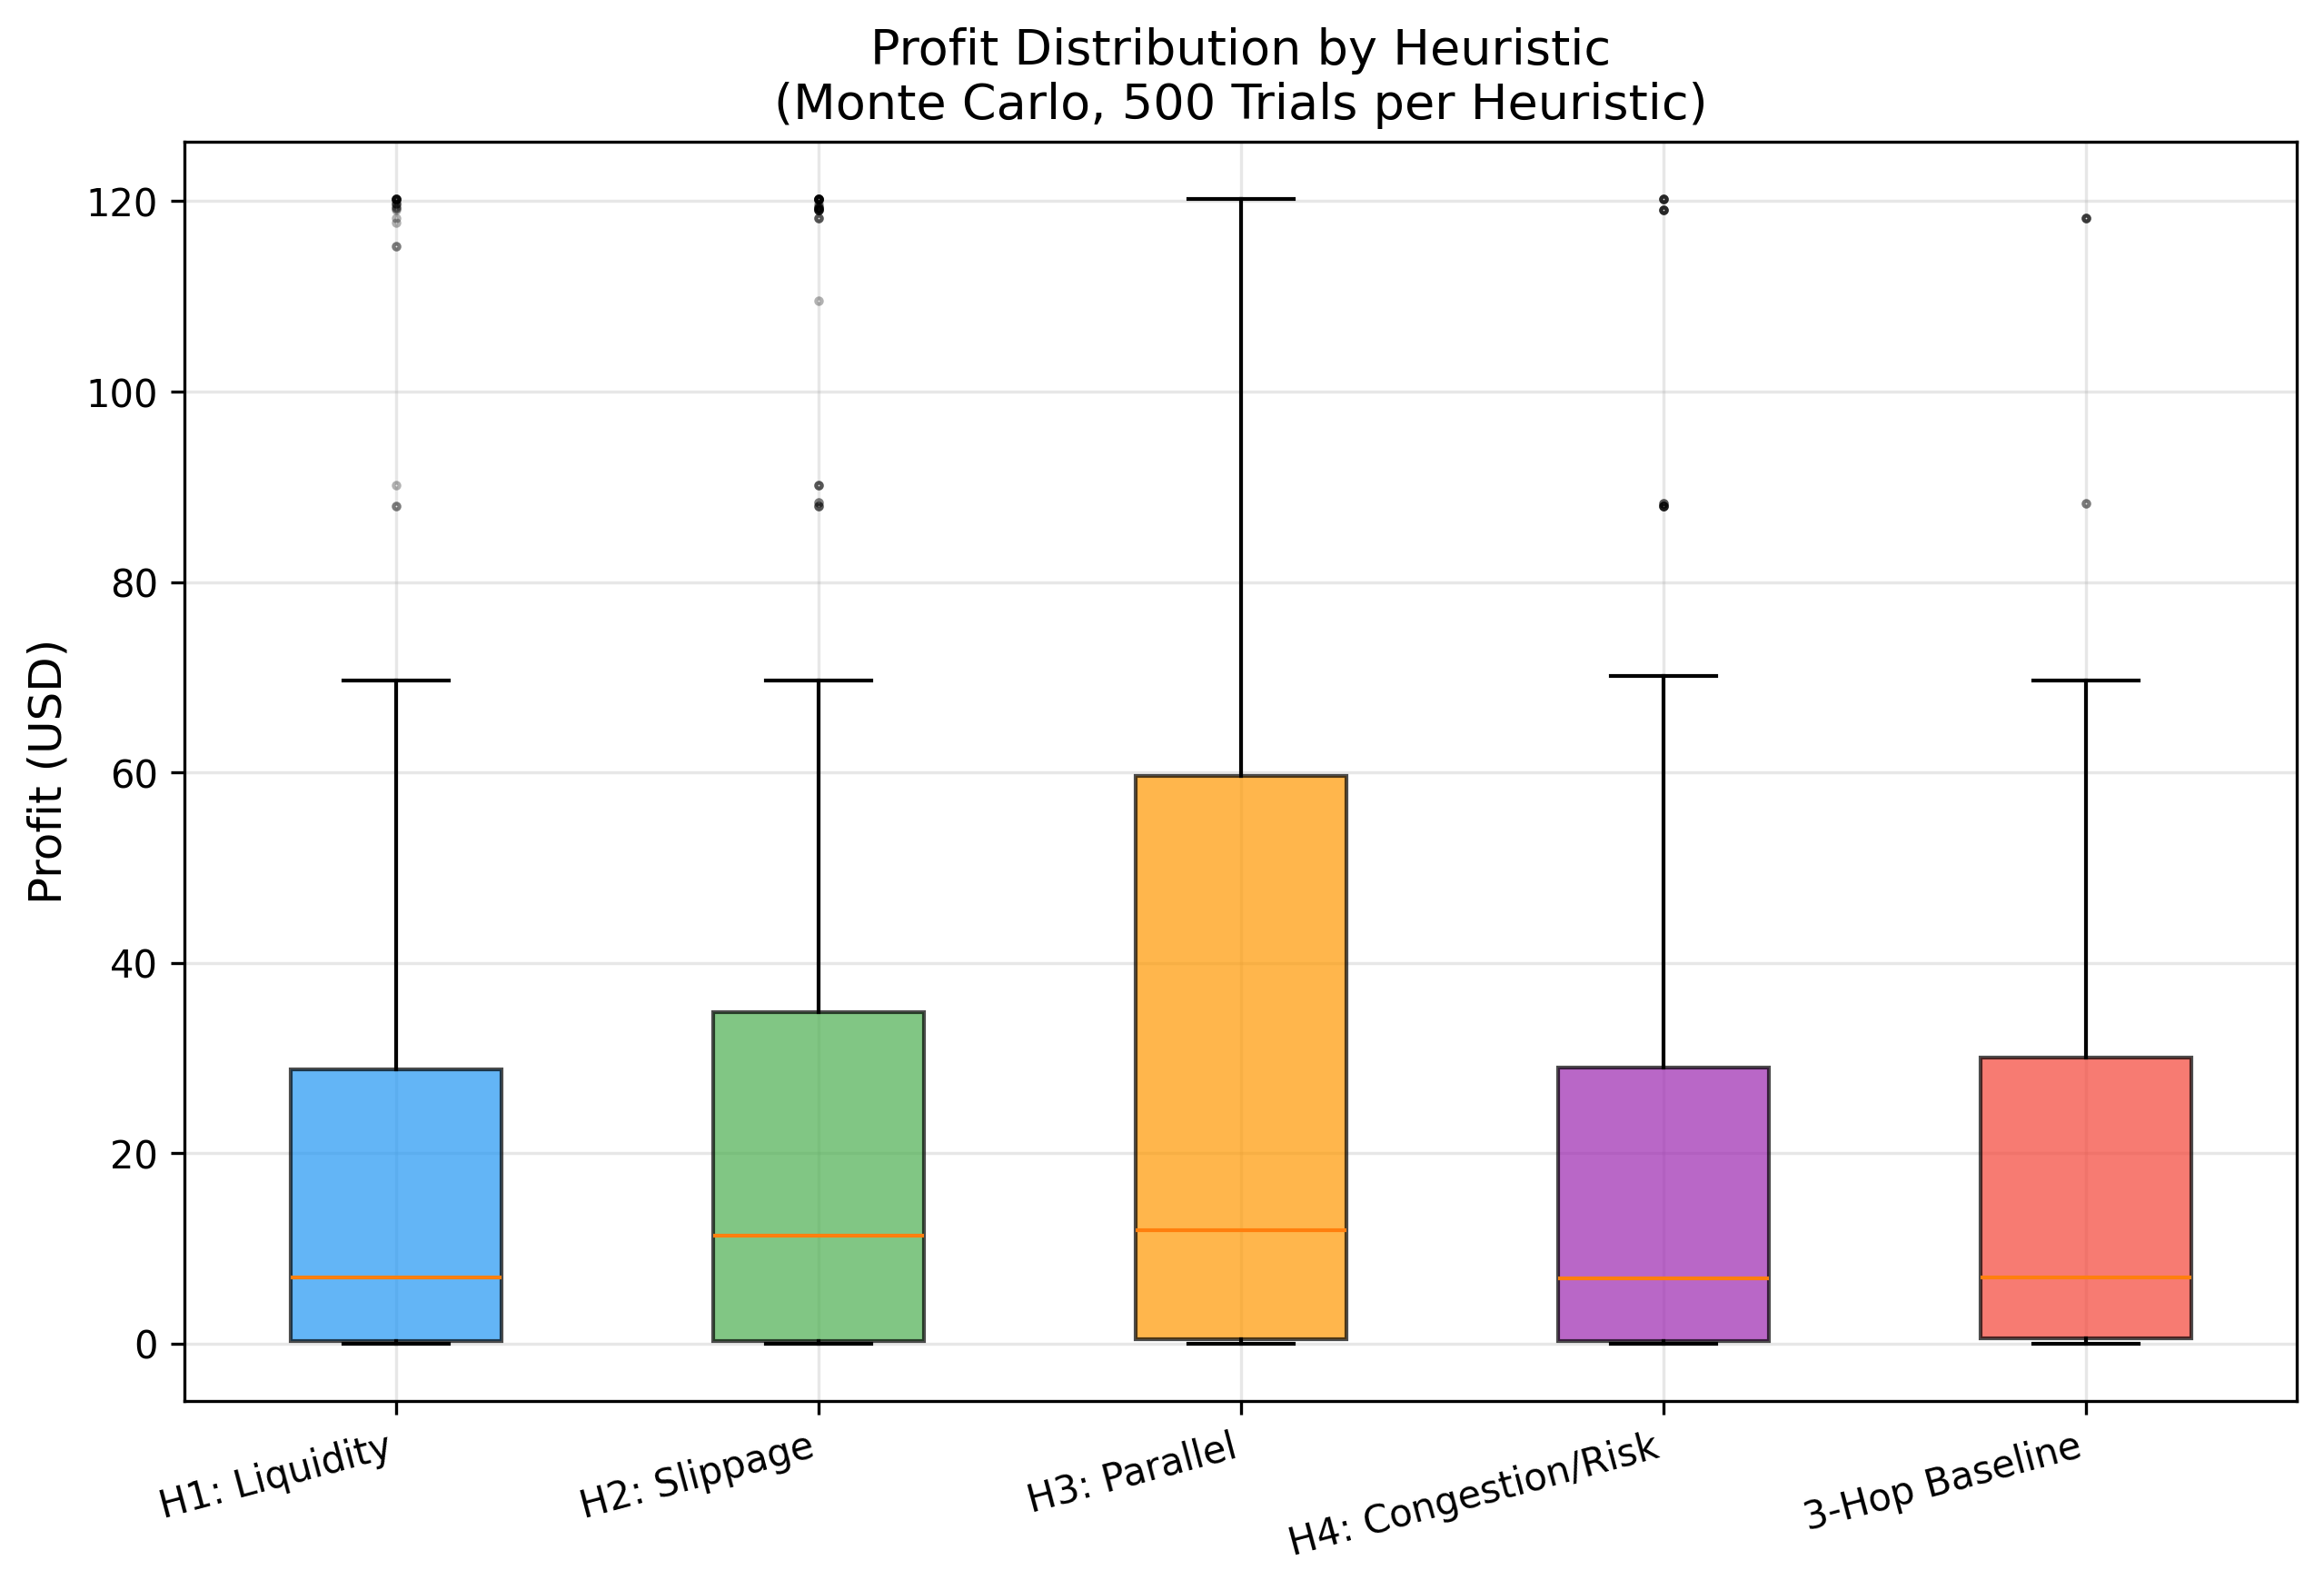
\includegraphics[width=\textwidth]{figures/fig03_profit_boxplot.png}
    \caption{Profit distribution by heuristic.}
\end{subfigure}
\caption{Overall heuristic performance summary.}
\label{fig:app_radar_profit}
\end{figure}

% ============================================================
% A.4 Interactive Visualization System
% ============================================================
\subsection{Interactive Visualization System}
\label{sec:streamlit_ui}

We provide a Streamlit-based web interface for real-time exploration of arbitrage opportunities. The UI integrates live CCXT market data and provides four tabs: (1)~\textbf{Arbitrage Graph} with interactive network visualization, heuristic selection, and search execution with streaming log output; (2)~\textbf{Live Prices} showing real-time stablecoin prices across exchanges; (3)~\textbf{Fees} displaying all fee structures; (4)~\textbf{Documentation}. Upon search completion, results include the complete route, per-node heuristic values, and step-by-step execution details with fees and transfer times. The system uses NetworkX for graph operations and Matplotlib for visualization. Source code is available in the anonymized repository.
